\apendice{Dossier técnico de programación}

\section{Introducción}
En este manual vamos a detallar de la forma más precisa posible, cómo reanudar este proyecto para que se pueda seguir con el desarrollo si así se desea.

\section{Estructura de directorios}
Este proyecto se encuentra con la siguiente distribución de carpetas:
\begin{itemize}
	\item
	\textbf{src:} se encuentra todo el código de la aplicación.
	\item
	\textbf{src/Interface:} contiene el código de la interfaz, tanto la página web como el convertidor y algunos ficheros de ejemplo.
	\item
	\textbf{src/Interface/subidas:} aloja los archivos subidos a la página web.
	\item
	\textbf{src/Interface/mygeodata:} almacena los archivos convertidos a GeoJSON y descomprimidos.
	\item
	\textbf{src/DattaLogger:} contiene el código que lleva incorporada la placa de desarrollo, encargado de almacenar las coordenadas en función del movimiento. 
	\item
	\textbf{Documentación:} nos encontramos con los PDF de la memoria y anexos, los archivos de \textit{latex} y las imágenes.
	\item
	\textbf{Selenium Test:} contiene los test creados con Selenium IDE para la interfaz.
	\item
	\textbf{Instalables:} contiene un link a todos los ejecutables que se han necesitado en el proyecto. (\textit{Kinetis}, \textit{Termite}, \textit{Python} y \textit{XAMPP}).
\end{itemize}

\section{Manual del programador}
\subsection{Instalación Kinetis Design Studio}
La primera parte del proyecto (la de la placa GPS) se ha desarrollado con la última versión de Kinetis (3.2.0) disponible en la página web oficial de NXP .
A continuación se aporta el enlace con la última versión:

\href{https://nxp.flexnetoperations.com/control/frse/product?entitlementId=402114997&lineNum=1&authContactId=115669057&authPartyId=124808297} {\texttt{https://nxp.flexnetoperations.com/control/frse/product...}}

\subsection{Instalación de Termite}
La terminal utilizada para visualizar los datos recogidos por la placa de desarrollo ha sido Termite en su versión 3.4 \textit{(complete setup)}. En el siguiente enlace encontraremos la última versión de Termite.

\url{https://www.compuphase.com/software_termite.htm}

\subsection{Instalación de Python}
Para poder ejecutar el archivo de conversión de forma local necesitaremos Python en nuestro ordenador. En este caso ha sido utilizado Python 3.7.0.
En el siguiente enlace podemos encontrar la última versión de Python disponible.

\href{http://www.oracle.com/technetwork/java/javase/downloads/javafxscenebuilder-1x-archive-2199384.html}{\texttt{http://www.oracle.com/technetwork/java/javase/downloads...}}

\subsection{Instalación de XAMPP}
Para poder ejecutar nuestra página en nuestro ordenador necesitaremos emular un servidor local, para lo que he utilizado XAMPP. Para  Además necesitaremos hacer algunos ajustes de configuración para que reconozca archivos Python (extensión .py). Voy a indicar el directorio por defecto, pero cada uno tendrá que ir a su directorio de instalación. 
\begin{itemize}
\tightlist
\item
	En el archivo de configuración C:\textbackslash{}xampp\textbackslash{}apache\textbackslash{}conf\textbackslash{}httpd.conf añadir la extensión .py en la línea del \textit{AddHandler} de forma que quede: AddHandler cgi-script .cgi .pl .asp .py
\item
	En la línea \textit{Options Indexes FollowSymLinks} debe tener la configuración \textit{ExecCGI}.
\item
	La primera línea de script de python debe ser la ruta a python.
\item
	Por último debemos reiniciar XAMPP para que se apliquen los cambios.
\end{itemize}

\imagen{configapache.PNG}{Cambios necesarios en los archivos de configuración sobre el manejador.}

\imagen{configapache2.PNG}{Inclusión de ExecCGI en las opciones.}

Para la ejecución local, debemos meter la carpeta \textit{interface} del proyecto en la carpeta de XAMPP \textit{htdocs}, en mi caso: \textit{C:\textbackslash{}xampp\textbackslash{}htdocs}
 
A continuación se encuentra el enlace a la página de Apache donde podremos descargar la última versión de XAMPP:
\url{https://www.apachefriends.org/es/download.html}

\section{Compilación, instalación y ejecución}

\subsection{Importar el proyecto en Kinetis}
Debemos descargar el proyecto exportado comprimido y subido a GitHub que contiene no solo el código fuente si no todos los componentes y la configuración: \url{https://github.com/alejandrolampreave/GPS}.
A continuación lo descomprimimos y ya podemos importarlo en Kinetis.

Para importar en Kinetis hacemos clic en \textit{File > Import}. Seguidamente seleccionamos la opción \textit{Existing Projects into Workspace} y seleccionamos la carpeta descomprimida. 
\imagen{import.PNG}{File>Import para importar nuestro proyecto a Kinetis.}

\imagen{import2.PNG}{Seleccionamos ``Existing Projects into Workspace''.}

%\begin{figure}[!h]
%	\centering
%	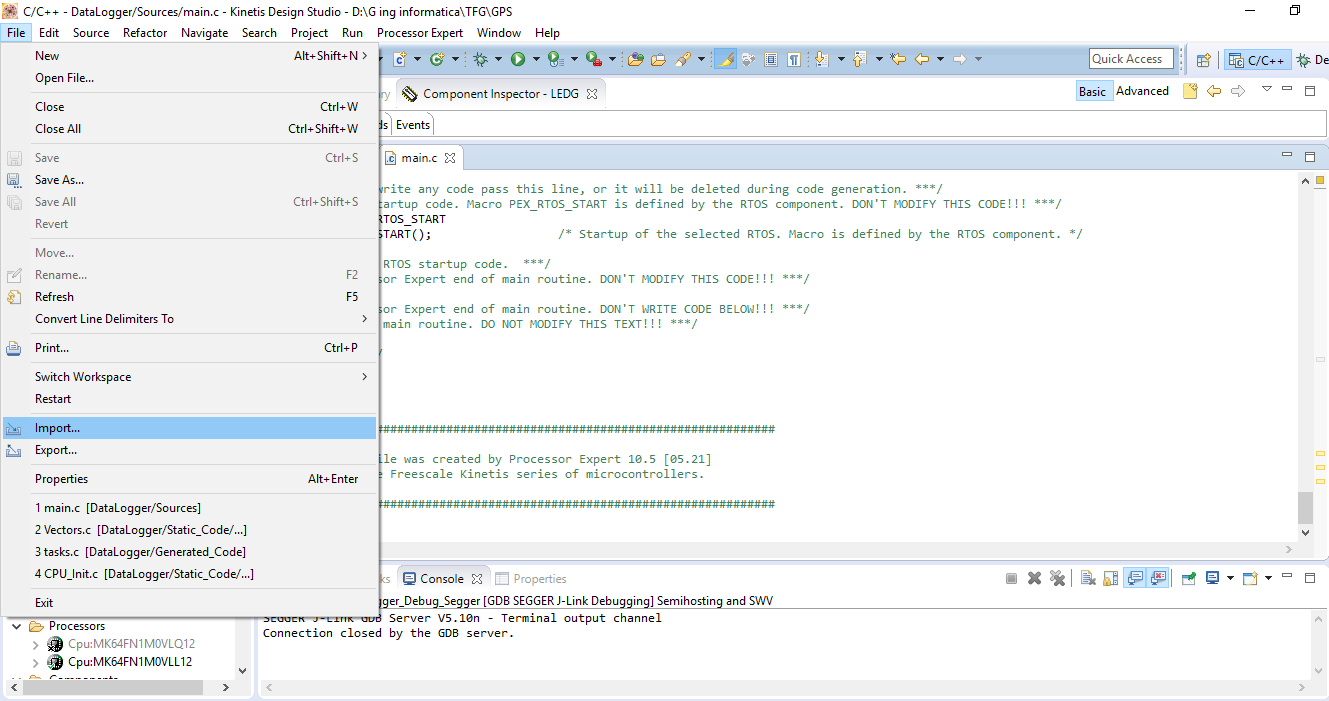
\includegraphics[width=0.8\textwidth, height=11.5cm]{import.PNG}
%	\caption{Importamos el proyecto a nuestro \textit{workspace} de .}\label{fig:import.png}
%\end{figure}
%\FloatBarrier
Ya podríamos empezar a trabajar en el proyecto.

\subsection{Grabar el programa en la placa}
Para grabar el programa en la placa de desarrollo tan solo debemos conectar la placa de desarrollo al conector de la placa de desarrollo OpenSDA y ejecutar nuestro programa dando al \textit{Run}, observando que la memoria seleccionada en ese momento sea la \textit{flash} y no la RAM.
\imagen{run.PNG}{Ejecutamos el programa para que quede almacenado en la memoria \textit{Flash} de la placa.}

\subsection{Ejecución}
Por último para ejecutar, solo tendremos que iniciar el servicio de Apache de XAMPP, abrir el navegador e introducir la siguiente url: \url{http://localhost/interface/index.html} para que se nos muestre la página de inicio de forma local. Una vez cargada podremos subir nuestro archivo, recogido por nuestro GPS y almacenado en la tarjeta microSD, para que se nos muestre en el mapa la ruta que hayamos hecho.
\imagen{apache.PNG}{Iniciamos el servicio de Apache.}

\section{Pruebas del sistema y calidad del código}
A lo largo de todo el desarrollo del proyecto se ha ido probando todo lo que se iba añadiendo para asegurarnos que no se perdiera ninguna funcionalidad a medida que avanzábamos. En caso de que diera algún error o algo no saliera según lo esperado, se replanteaba lo que se quería implementar y se buscaban posibles soluciones dentro de la misma opción o se pensaba en una alternativa válida.

Tanto desde el punto de vista del usuario como para nosotros mismos se habilitó el \textit{led} rgb de la placa de forma que nos indicase en todo momento qué estaba haciendo, \textit{led} verde obtención de coordenadas, \textit{led} rojo escritura en tarjeta. Además se ha comprobado que únicamente se permita la subida de archivos con extensión .txt, que es como se almacenan en la tarjeta.

De forma adicional se ha hecho uso de la herramienta de Selenium IDE, con la cual se ha desarrollado un pequeño test que comprobase la carga de los diferentes bloques de la página, incluyendo el mapa final. Se adjuntan los test junto con el proyecto.
\imagen{test.PNG}{Test realizado mediante Selenium IDE.}

En la última fase del proyecto se realizó una prueba en un ambiente real, dentro de un coche con la placa de desarrollo, para que registrara la ruta. Luego se introdujo la tarjeta en el ordenador y se subió a la página web, mostrando de forma satisfactoria la ruta seguida.

En cuanto a la calidad del código se refiere barajamos varias herramientas, entre ellas: SonarQube, Codacy, CodeClimate y CodeBeat. Finalmente seleccionamos SonarQube por ser una de las más importantes y que mejor se adaptaba al proyecto. En su página web seleccionamos el método \textit{online}, nos redireccionó a una página llamada Sonarcloud y tras descargarnos el ``sonar-scanner-3.3.0.1492'' ejecutamos un comando que nos dieron para generar el análisis. Cabe destacar que solo hemos podido pasar el escáner a los archivos de la interfaz, ya que al pasar el \textit{build wraper} proporcionado por la herramienta por nuestros ficheros fuentes en C no los reconocía. Diría que es porque la \textit{Build Tool} utilizado en Kinetis no es GCC si no uno específico llamado \textit{Cross ARM GCC}. 

Obtuvimos buenos resultados pero tras unas pequeñas mejoras, incluyendo algunas de la plantilla HTML utilizada, conseguimos mejorar la calidad de nuestro código sustancialmente. Algunos de los errores fueron marcados como falsos positivos, pero fueron acompañados por una explicación en tal caso. El link para comprobar la calidad del código es: \url{https://sonarcloud.io/dashboard?id=alejandrolampreave_GPS}
\imagen{sonarcloud1.PNG}{Escaneo realizado antes de corregir el código.}
\imagen{sonarcloud2.PNG}{Escaneo realizado tras corregir la mayoría de errores.}



